\documentclass[border=12pt]{standalone}
\usepackage[utf8]{inputenc}
\usepackage{amsmath}
\usepackage{tikz}
\usetikzlibrary{arrows.meta, positioning, calc, shapes.geometric, backgrounds}

\definecolor{espblue}{RGB}{28, 78, 148}
\definecolor{espgray}{RGB}{45, 52, 54}
\definecolor{pcbgreen}{RGB}{20, 110, 60}
\definecolor{goldpin}{RGB}{218, 165, 32}
\definecolor{wiregreen}{RGB}{46, 204, 113}
\definecolor{wirered}{RGB}{231, 76, 60}
\definecolor{wireblack}{RGB}{44, 62, 80}
\definecolor{wireorange}{RGB}{230, 126, 34}
\definecolor{wirepurple}{RGB}{142, 68, 173}
\definecolor{wireblue}{RGB}{41, 128, 185}
\definecolor{wireyellow}{RGB}{241, 196, 15}

\begin{document}
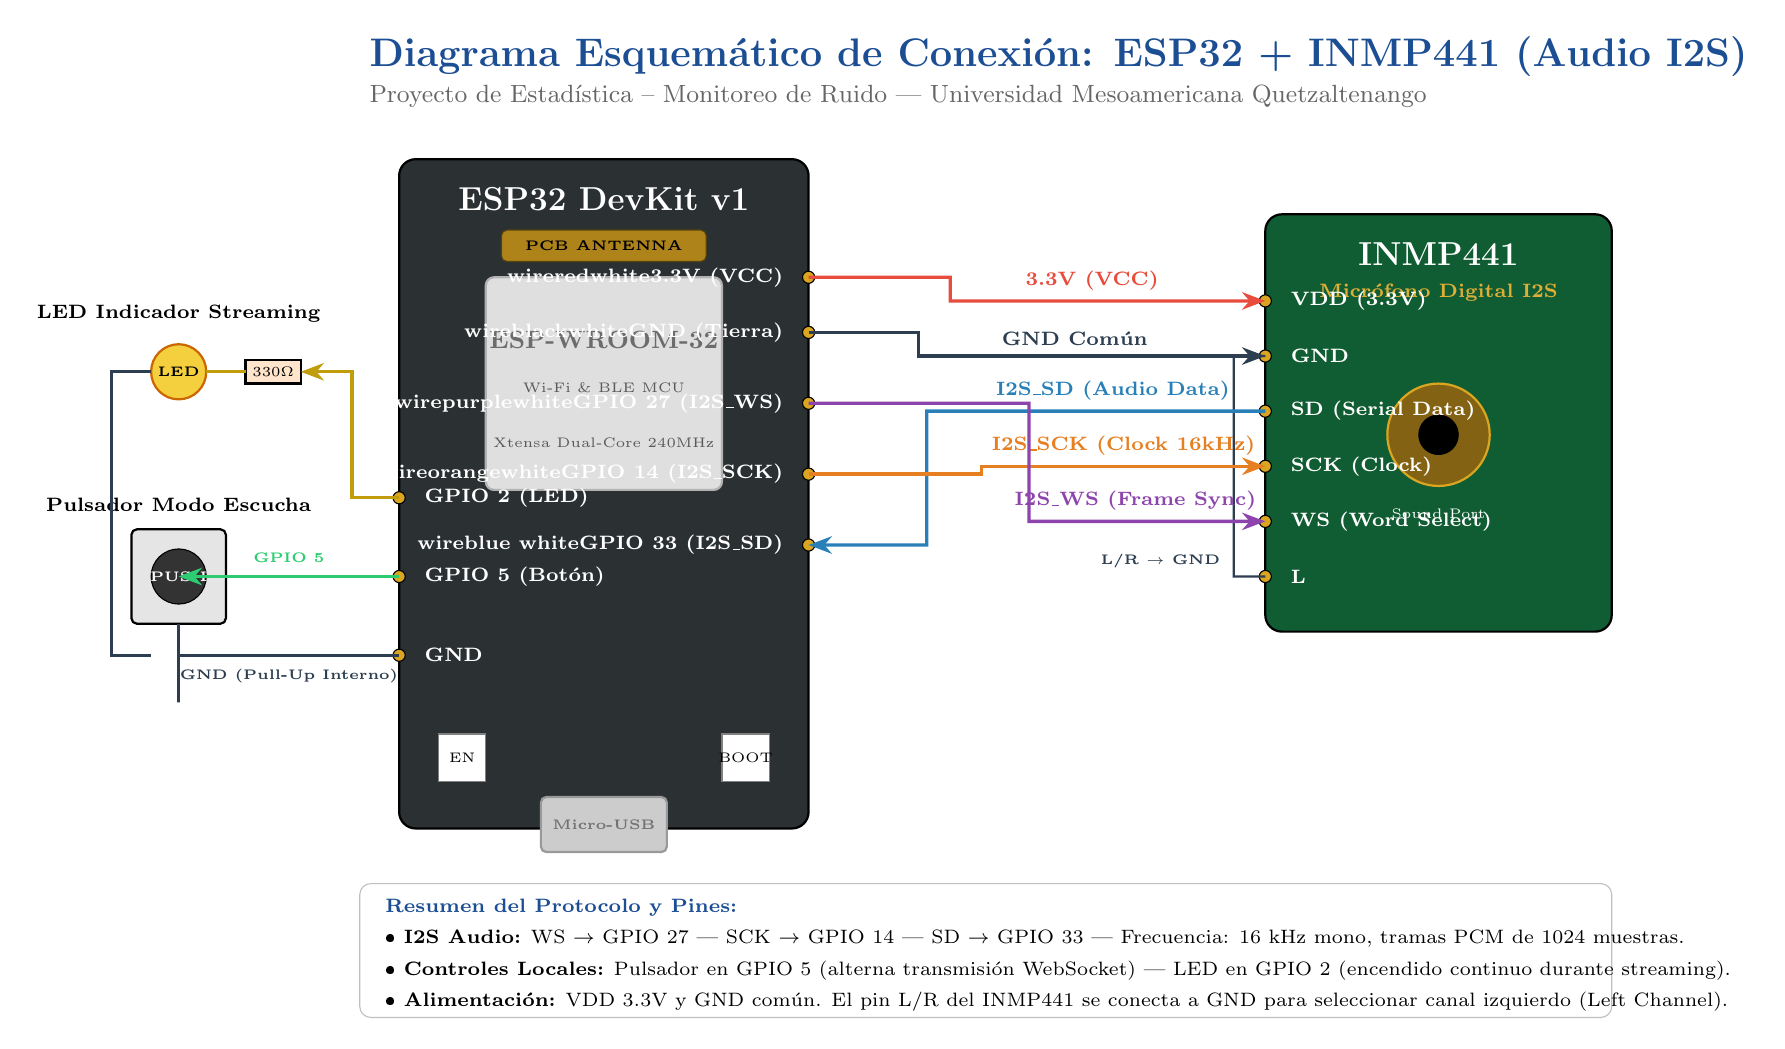
\begin{tikzpicture}[font=\sffamily, scale=1.0, >=Stealth]

    % =========================================================================
    % TÍTULO Y ENCABEZADO
    % =========================================================================
    \node[anchor=west, font=\bfseries\Large, text=espblue] at (-0.5, 9.8) {Diagrama Esquemático de Conexión: ESP32 + INMP441 (Audio I2S)};
    \node[anchor=west, font=\small, text=gray!80!black] at (-0.5, 9.3) {Proyecto de Estadística -- Monitoreo de Ruido | Universidad Mesoamericana Quetzaltenango};

    % =========================================================================
    % 1. MÓDULO ESP32 DEVKIT
    % =========================================================================
    % Placa PCB principal
    \draw[fill=espgray!95!black, draw=black, thick, rounded corners=6pt] (0, 0) rectangle (5.2, 8.5);
    \node[font=\bfseries\large, text=white] at (2.6, 8.0) {ESP32 DevKit v1};
    
    % Antena PCB dorada
    \draw[fill=goldpin!80!black, draw=goldpin!40!black, rounded corners=2pt] (1.3, 7.2) rectangle (3.9, 7.6);
    \node[font=\tiny\bfseries, text=black] at (2.6, 7.4) {PCB ANTENNA};

    % Chip metálico ESP-WROOM-32
    \draw[fill=gray!25, draw=gray!60, thick, rounded corners=3pt] (1.1, 4.3) rectangle (4.1, 7.0);
    \node[font=\small\bfseries, text=gray!85!black] at (2.6, 6.2) {ESP-WROOM-32};
    \node[font=\tiny, text=gray!70!black] at (2.6, 5.6) {Wi-Fi \& BLE MCU};
    \node[font=\tiny, text=gray!70!black] at (2.6, 4.9) {Xtensa Dual-Core 240MHz};

    % Conector Micro-USB
    \draw[fill=gray!40, draw=gray!80, thick, rounded corners=2pt] (1.8, -0.3) rectangle (3.4, 0.4);
    \node[font=\tiny\bfseries, text=gray!90!black] at (2.6, 0.05) {Micro-USB};

    % Botones EN y BOOT
    \draw[fill=white, draw=gray] (0.5, 0.6) rectangle (1.1, 1.2);
    \node[font=\tiny] at (0.8, 0.9) {EN};
    \draw[fill=white, draw=gray] (4.1, 0.6) rectangle (4.7, 1.2);
    \node[font=\tiny] at (4.4, 0.9) {BOOT};

    % Pines del costado derecho (usados para I2S y alimentación)
    \coordinate (P_3V3)  at (5.2, 7.0);
    \coordinate (P_GND)  at (5.2, 6.3);
    \coordinate (P_D27)  at (5.2, 5.4);
    \coordinate (P_D14)  at (5.2, 4.5);
    \coordinate (P_D33)  at (5.2, 3.6);

    % Pines del costado izquierdo (usados para Pulsador y LED)
    \coordinate (P_D5)   at (0.0, 3.2);
    \coordinate (P_D2)   at (0.0, 4.2);
    \coordinate (P_GNDL) at (0.0, 2.2);

    % Etiquetas de pines derechos
    \foreach \coord/\label/\color in {
        P_3V3/3.3V (VCC)/wirered,
        P_GND/GND (Tierra)/wireblack,
        P_D27/GPIO 27 (I2S\_WS)/wirepurple,
        P_D14/GPIO 14 (I2S\_SCK)/wireorange,
        P_D33/GPIO 33 (I2S\_SD)/wireblue
    } {
        \draw[fill=goldpin, draw=black] (\coord) circle (2.2pt);
        \node[anchor=east, font=\scriptsize\bfseries, text=white] at ($(\coord)+(-0.2, 0)$) {\label};
    }

    % Etiquetas de pines izquierdos
    \draw[fill=goldpin, draw=black] (P_D2) circle (2.2pt);
    \node[anchor=west, font=\scriptsize\bfseries, text=white] at ($(P_D2)+(0.2, 0)$) {GPIO 2 (LED)};

    \draw[fill=goldpin, draw=black] (P_D5) circle (2.2pt);
    \node[anchor=west, font=\scriptsize\bfseries, text=white] at ($(P_D5)+(0.2, 0)$) {GPIO 5 (Botón)};

    \draw[fill=goldpin, draw=black] (P_GNDL) circle (2.2pt);
    \node[anchor=west, font=\scriptsize\bfseries, text=white] at ($(P_GNDL)+(0.2, 0)$) {GND};


    % =========================================================================
    % 2. MÓDULO SENSOR INMP441 (MEMS I2S)
    % =========================================================================
    \draw[fill=pcbgreen!85!black, draw=black, thick, rounded corners=6pt] (11.0, 2.5) rectangle (15.4, 7.8);
    \node[font=\bfseries\large, text=white] at (13.2, 7.3) {INMP441};
    \node[font=\scriptsize\bfseries, text=goldpin!90!white] at (13.2, 6.8) {Micrófono Digital I2S};

    % Puerto acústico (círculo dorado central)
    \draw[fill=goldpin!60!black, draw=goldpin, thick] (13.2, 5.0) circle (0.65);
    \draw[fill=black] (13.2, 5.0) circle (0.25);
    \node[font=\tiny, text=white] at (13.2, 4.0) {Sound Port};

    % Pines de conexión del INMP441 (costado izquierdo)
    \coordinate (M_VDD) at (11.0, 6.7);
    \coordinate (M_GND) at (11.0, 6.0);
    \coordinate (M_SD)  at (11.0, 5.3);
    \coordinate (M_SCK) at (11.0, 4.6);
    \coordinate (M_WS)  at (11.0, 3.9);
    \coordinate (M_LR)  at (11.0, 3.2);

    \foreach \coord/\label in {
        M_VDD/VDD (3.3V),
        M_GND/GND,
        M_SD/SD (Serial Data),
        M_SCK/SCK (Clock),
        M_WS/WS (Word Select),
        M_LR/L/R (Canal Izq)
    } {
        \draw[fill=goldpin, draw=black] (\coord) circle (2.2pt);
        \node[anchor=west, font=\scriptsize\bfseries, text=white] at ($(\coord)+(0.2, 0)$) {\label};
    }

    % Conexión puente interna L/R a GND en el sensor
    \draw[thick, wireblack] (M_LR) -- ++(-0.4, 0) -- ++(0, 2.8) -- (M_GND);
    \node[font=\tiny\bfseries, text=wireblack, anchor=east] at (10.55, 3.4) {L/R $\rightarrow$ GND};


    % =========================================================================
    % 3. CABLEADO I2S Y ALIMENTACIÓN (ESP32 <--> INMP441)
    % =========================================================================
    % VDD (3.3V) - Rojo
    \draw[very thick, wirered, ->] (P_3V3) -- ++(1.8, 0) -- ++(0, -0.3) -- (M_VDD)
        node[pos=0.45, above, font=\scriptsize\bfseries, text=wirered] {3.3V (VCC)};

    % GND - Negro
    \draw[very thick, wireblack, ->] (P_GND) -- ++(1.4, 0) -- ++(0, -0.3) -- (M_GND)
        node[pos=0.45, above, font=\scriptsize\bfseries, text=wireblack] {GND Común};

    % SD (Serial Data) - Azul
    \draw[very thick, wireblue, <-] (P_D33) -- ++(1.5, 0) -- ++(0, 1.7) -- (M_SD)
        node[pos=0.55, above, font=\scriptsize\bfseries, text=wireblue] {I2S\_SD (Audio Data)};

    % SCK (Clock) - Naranja
    \draw[very thick, wireorange, ->] (P_D14) -- ++(2.2, 0) -- ++(0, 0.1) -- (M_SCK)
        node[pos=0.5, above, font=\scriptsize\bfseries, text=wireorange] {I2S\_SCK (Clock 16kHz)};

    % WS (Word Select) - Púrpura
    \draw[very thick, wirepurple, ->] (P_D27) -- ++(2.8, 0) -- ++(0, -1.5) -- (M_WS)
        node[pos=0.45, above, font=\scriptsize\bfseries, text=wirepurple] {I2S\_WS (Frame Sync)};


    % =========================================================================
    % 4. COMPONENTES EXTERNOS (PULSADOR Y LED)
    % =========================================================================
    % Pulsador Push Button (GPIO 5)
    \coordinate (BTN_POS) at (-2.8, 3.2);
    \draw[fill=gray!20, draw=black, thick, rounded corners=2pt] ($(BTN_POS)+(-0.6, -0.6)$) rectangle ($(BTN_POS)+(0.6, 0.6)$);
    \draw[fill=black!80] (BTN_POS) circle (0.35);
    \node[font=\tiny\bfseries, text=white] at (BTN_POS) {PUSH};
    \node[font=\scriptsize\bfseries, text=black, anchor=south] at ($(BTN_POS)+(0, 0.7)$) {Pulsador Modo Escucha};

    % Conexión del Pulsador al ESP32 (GPIO 5 y GND)
    \draw[very thick, wiregreen, ->] (P_D5) -- (BTN_POS);
    \draw[very thick, wireblack] ($(BTN_POS)+(0, -0.6)$) -- ++(0, -1.0) -- ($(P_GNDL)+(-2.8, 0)$) -- (P_GNDL);
    \node[font=\tiny\bfseries, text=wiregreen, anchor=south] at (-1.4, 3.25) {GPIO 5};
    \node[font=\tiny\bfseries, text=wireblack, anchor=north] at (-1.4, 2.15) {GND (Pull-Up Interno)};

    % Diodo LED Indicador (GPIO 2)
    \coordinate (LED_POS) at (-2.8, 5.8);
    \draw[fill=wireyellow!80!white, draw=orange!80!black, thick] (LED_POS) circle (0.35);
    \node[font=\tiny\bfseries, text=black] at (LED_POS) {LED};
    \node[font=\scriptsize\bfseries, text=black, anchor=south] at ($(LED_POS)+(0, 0.5)$) {LED Indicador Streaming};

    % Resistencia limitadora 330 ohm
    \coordinate (R_POS) at (-1.6, 5.8);
    \draw[fill=orange!20!white, draw=black, thick] ($(R_POS)+(-0.35, -0.15)$) rectangle ($(R_POS)+(0.35, 0.15)$);
    \node[font=\tiny\bfseries] at (R_POS) {$330\Omega$};

    % Conexiones del LED
    \draw[very thick, wireyellow!80!black, ->] (P_D2) -- ++(-0.6, 0) -- ++(0, 1.6) -- ($(R_POS)+(0.35, 0)$);
    \draw[very thick, wireyellow!80!black] ($(R_POS)+(-0.35, 0)$) -- ($(LED_POS)+(0.35, 0)$);
    \draw[very thick, wireblack] ($(LED_POS)+(-0.35, 0)$) -- ++(-0.5, 0) -- ++(0, -3.6) -- ++(0.5, 0);


    % =========================================================================
    % 5. CAJA DE LEYENDA TÉCNICA
    % =========================================================================
    \draw[fill=white, draw=gray!50, rounded corners=4pt, thin] (-0.5, -2.4) rectangle (15.4, -0.7);
    \node[anchor=west, font=\scriptsize\bfseries, text=espblue] at (-0.3, -1.0) {Resumen del Protocolo y Pines:};
    \node[anchor=west, font=\scriptsize] at (-0.3, -1.4) {• \textbf{I2S Audio:} WS $\rightarrow$ GPIO 27 | SCK $\rightarrow$ GPIO 14 | SD $\rightarrow$ GPIO 33 | Frecuencia: $16\text{ kHz}$ mono, tramas PCM de 1024 muestras.};
    \node[anchor=west, font=\scriptsize] at (-0.3, -1.8) {• \textbf{Controles Locales:} Pulsador en GPIO 5 (alterna transmisión WebSocket) | LED en GPIO 2 (encendido continuo durante streaming).};
    \node[anchor=west, font=\scriptsize] at (-0.3, -2.2) {• \textbf{Alimentación:} VDD $3.3\text{V}$ y GND común. El pin L/R del INMP441 se conecta a GND para seleccionar canal izquierdo (Left Channel).};

\end{tikzpicture}
\end{document}
